\documentclass[11pt, a4paper]{COMP3711}
\usepackage{verbatim}
\usepackage{fancyhdr}
\usepackage{booktabs}
\usepackage{setspace}
\usepackage{amsmath,mathrsfs}
\usepackage{multicol}
\usepackage{amssymb}
\usepackage{graphicx}
\usepackage{caption}
\usepackage{subcaption}
\usepackage{array}
\usepackage{xcolor}
\usepackage{float}
\usepackage{enumitem}
\usepackage{tabularx}
\usepackage{wasysym}
\usepackage{pbox}
\usepackage{tikz}
\usepackage{mathtools}
\usetikzlibrary{matrix}
\usepackage[normalem]{ulem}
\usepackage{multirow}
\usepackage[linesnumbered, ruled, boxed]{algorithm2e}
\SetKwRepeat{Do}{do}{while}

\title{Topic 3}
\subtitle{Randomized Algorithms}

\begin{document}
\begin{spacing}{1.5}
    
    \section{Recap: Probability}

    {\bf Expectation: } $\disp \E(X)=\sum i\cdot \Pr(X=i)$

    {\bf Linearity of expectation: } $\E(X+Y)=\E(X)+\E(Y)$, 
    no matter $X$ and $Y$ are independent or not.

    {\bf Indicator random variables:} $X$ only takes 
    0 or 1, which means $\E(X)=\Pr(X=1)$.

    Example 1: coin comes up heads with probability $p$ and 
    tails with $1-p$. Find the expectation of flips $X$ 
    until first head is seen.
    \begin{align*}
        \E(X)&=\sum_{j=1}^{\infty} j\cdot \Pr(X=j)\\
        &= \sum_{j=1}^{\infty}j\cdot (1-p)^{j-1}\cdot p\\
        &= \frac{p}{1-p} \sum_{j=1}^{\infty}j\cdot (1-p)^{j}\\
        &= \frac{p}{1-p}\cdot \frac{1-p}{p} =\frac{1}{p}
    \end{align*}

    The last step is somehow mysterious, the brief idea is: 
    $$\left(\sum_{n=1}^{\infty} x^i\right)'=\sum_{n=1}^{\infty}i\cdot x^{i-1}$$

    multiply each side by $x$, and notice the left hand side is the 
    derivative of geometric series, then: 
    $$x\cdot \left(\frac{x}{1-x}\right)'=\sum_{n=1}^{\infty}i\cdot x^{i}$$
    This gives the last step above.

    Example 2: Roll two dice. What is the expected total value $X$?

    It is trivial that $\E(X_1)=\E(X_2)=3.5$, then: 
    $$\E(X_1+X_2)=\E(X_1)+\E(X_2)=7$$

    \section{The Hiring Problem}

    Consider we're looking for an assistant and there are $n$ 
    candidates. We would like to hire the best one, so we 
    interview one by one, and if the current one is better than 
    the best one we've seen before, we just fire the previous one 
    and hire the current one.

    \begin{algorithm*}
        \caption{Hire-Assistant($n$)}

        $best\lar 0$

        \For{$i\lar 1$ to $n$}{
            interview candidate $i$

            \If{candidate $i$ is better than $best$}{
                fire $best$

                hire candidate $i$

                $best\lar i$
            }
        }
    \end{algorithm*}

    This algorithm runs fine, but there is one problem that we 
    may hire too many people(worst case $n$) 
    before we finally find the best one,
    so it may cost lots of money to fire old ones.
    In order to make things better, we consider interview the 
    candidates {\it in a random order}.

    \begin{algorithm*}
        \caption{Hire-Assistant($n$)}

        {\blue{randomly permute all $n$ candidates}}

        $best\lar 0$

        \For{$i\lar 1$ to $n$}{
            interview candidate $i$

            \If{candidate $i$ is better than $best$}{
                fire $best$

                hire candidate $i$

                $best\lar i$
            }
        }
    \end{algorithm*}

    So what is the expected number of hires in the algorithm above?
    Let an indicator variable $X_i$ where: 
    $$X_i=\left\{ 
        \setstretch{0.5}
        \begin{array}{ll}
            1 &, \text{if we hire candidate }i\\
            0 &, \text{if we don't}
        \end{array}
     \right.$$
    
    Then apparently the number of hires $X=X_1+\cdots+X_n$, thus 
    the expected number of hires, $\E(X)=\E(X_1)+\cdots+\E(X_n)$ 
    according to the linearity of expectation.

    Then what is $\E(X_i)$? Since $X_i$ is an indicator variable, 
    $\E(X_i)=\Pr(X_i=1)$. We hire the candidate $i$ if and only 
    if he/she is the best among all first $i$ candidates, and 
    since they are arranged randomly, the probability that the best 
    one among first $i$ candidates is at the last position is $\frac{1}{i}$.
    Thus, $\E(X_i)=\frac{1}{i}$, and 
    $$\E(X)=\E(X_1)+\cdots+\E(X_n)=1+\frac{1}{2}+\cdots+\frac{1}{n-1}+\frac{1}{n}
    =\Theta(\log n)$$

    \section{Generating a random permutation}

    Notice that in the hiring problem above, we first need to randomly
    permute those candidates. But how can we do that? 
    (Here randomly means all permutations, in total $n!$, should 
    appear with equal probability $\frac{1}{n!}$)

    Let's first look at the implementation of this algorithm, and 
    then explain why it can perform the job well. 
    Assume out computer has a procedure $Random(i, j)$ that can  
    generates a {\bf random uniform} integer between $i$ and $j$.
    ({\bf uniform} means each int occurs with same probability)

    \begin{algorithm*}
        \caption{RandomPermute($A$)}

        $n\lar A.length$

        \For{$i\lar 1$ to $n$}{
            swap $A[i]$ with $A[Random(1, i)]$
        }
    \end{algorithm*}

    \begin{center}
        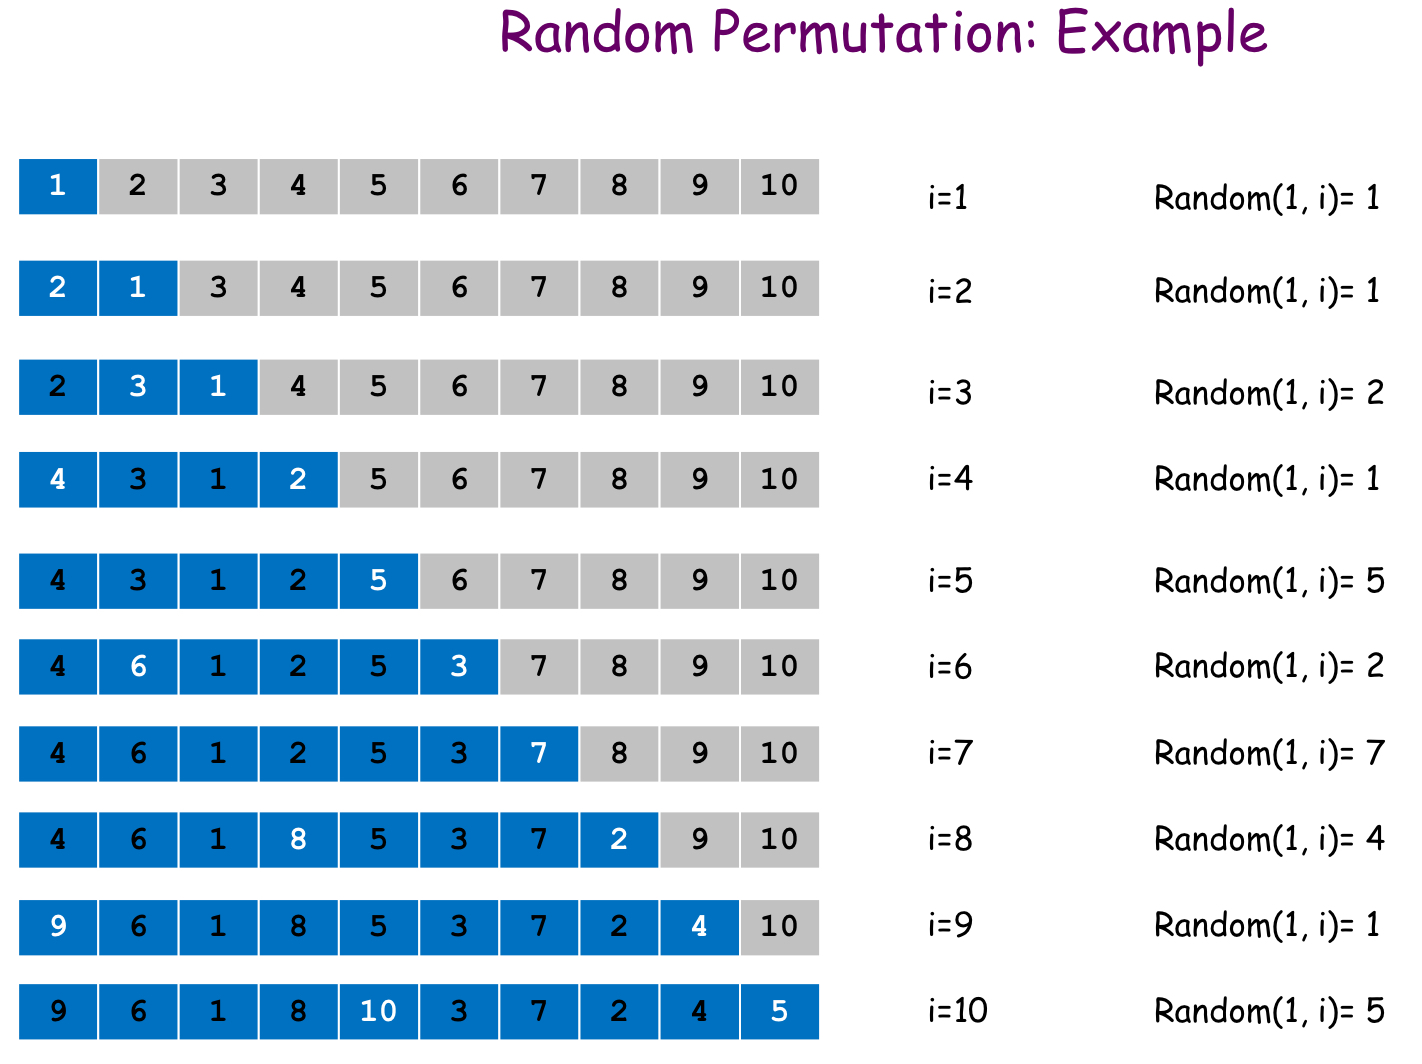
\includegraphics[scale=0.2]{images/03-permutation-eg.jpeg}
    \end{center}

    In the example above, take the last step as an example, 
    the random number we generated is 5, so we will 
    swap the item at index 5, which is 5, with the last item 
    10. Then 10 ends up with index 5 and 5 ends up with index 10.

    Notice this process is actually {\it revertible}, 
    from the end to beginning. For example, we notice at the end, 
    $A[5]=10$, so the last step we must have swapped $A[5]$ with 
    $A[10]$, since before last step, $A[10]=10$. Then if we 
    ``revert'' this step, i.e., swap $A[5]$ and $A[10]$, then 
    the array will back to the status before last step.

    Then, if we denote the random number generated at step $i$
    to be $r_i$, the $n$-tuple $(r_1,\cdots, r_n)$ will 
    generate a permutation of the array. Moreover, given the 
    result permutation, we can actually ``revert'' the process, 
    like we discussed above, to get the $(r_1,\cdots,r_n)$ 
    generated. This means, a tuple $(r_1,\cdots, r_n)$ is 
    {\bf uniquely corresponding} to a permutation at last.
    So if two tuples are different, the permutations they 
    generate are different as well!

    Now we can easily prove the correctness of this algorithm, 
    since each tuple is generated with probability $\dfrac{1}{n!}$,
    (each $r_i$ is generated with probability $\dfrac{1}{n}$),
    then each permutation is also generated with probability 
    $\dfrac{1}{n!}$.

    \vspace{0.3in}

    Here we will give another proof by induction, to show 
    that ``after the $i$-th iteration, $A[1\cdots i]$
    has been randomly permuted.''

    {\bf Base case: }$i=1$, trivial.

    {\bf Inductive step:} Assume $A[1\cdots i-1]$ has been randomly 
    permuted after $i-1$ iterations of the algorithm, then 
    we will calculated the probability that $A[1\cdots i]=
    (a_1,\cdots,a_i)$ appears after the $i$-th iteration.

    For example, if $i=10$, then after $(i-1)$ steps, 
    the array must be something like this: 
    $$[2,8,{\blue 7},3,4,1,5,6,9,{\blue 10}]$$
    then what is the probability that we generate 
    $[2,8,{\blue 10},3,4,1,5,6,9,{\blue 7}]$ after $i$-th step? 
    We must swap $A[3]=7$ with $A[10]=10$, which means 
    $Random(1, i)$ must return 3 to achieve that.

    To summarize the above paragraph, we can get 
    $A[1\cdots i]=(a_1,\cdots,a_i)$ after $i$-th iteration 
    {\it if and only if}
    \begin{itemize}
        \item $Random(1,i)$ returns a specific number and 
        \item $A[1\cdots i-1]$ is a specific $(a_1,\cdots,a_{i-1})$
    \end{itemize}

    The second point above has a probability $\dfrac{1}{(i-1)!}$ according 
    to assumption of induction, the first point above has a probability 
    $\dfrac{1}{i}$. Hence, the probability that $A[1\cdots i]=(a_1,\cdots,a_i)$
    is $\dfrac{1}{(n-1)!}\cdot \dfrac{1}{i}=\dfrac{1}{i!}$, which 
    means that it's a random permutation.

    \section{Quick Sort}

    {\bf Quick Sort} is somehow similar to {\bf Merge Sort}. Instead, 
    it chooses a {\bf pivot} each time, and then {\bf partitions}
    the array so that all items less than or equal to the pivot are 
    on the left and all items greater than pivot are 
    on the right.

    Then it recursively calls QuickSort to left and right sides.

    \begin{algorithm*}
        \caption{QuickSort($A$, $l$, $r$)}

        \If{$l\ge r$}{
            return
        }
        $pivot\lar $ Partition($A$, $l$, $r$)

        QuickSort($A$, $l$, $pivot - 1$)\qquad \tcp{quick sort left part}

        QuickSort($A$, $pivot+1$, $r$)\qquad \tcp{quick sort right part}
    \end{algorithm*}

    For the {\bf Partition} process, we need to choose a pivot first, 
    here we simply choose the last element as pivot. 
    Then we divide the array $A[l\cdots r]$ into two parts: 
    $A[l\cdots i]$ are all smaller or equal than pivot $A[r]$, $A[i+1\cdots j-1]$
    are all larger than pivot $A[r]$, while $A[j\cdots r-1]$ 
    are not decided yet.

    To divide, we perform ``swaps'': iterate $j$ from $l$ to $r-1$,
    if $A[j]$ is smaller or equal than pivot $A[r]$, we expand 
    the area of left part, i.e., $i\lar i+1$, and then swap 
    $A[j]$ with $A[i]$. This will enlarge smaller subpart by size 1, 
    and put the newly found item into that part.
    On the contrary, if $A[j]$ is larger than pivot, then we 
    just expand the larger subpart by size 1, say $j\lar j+1$,
    and no need to do other stuff since $A[j]$ will be already 
    contained after we expand the part.

    Here is the implementation of this process: 

    \begin{algorithm*}
        \caption{Partition($A$, $l$, $r$)}

        $x\lar A[r]$ \qquad \tcp{choose last item to be pivot}

        $i\lar l - 1$\qquad \tcp{No item found yet, so there should be nothing in $A[l\cdots i]$}

        \For{$j\lar l$ to $r-1$}{
            \If{$A[j]\le x$}{
                $i\lar i + 1$   \qquad \tcp{expand left part}

                swap $A[i]$ and $A[j]$ \qquad \tcp{include the new item into left part}
            }
        }
        swap $A[i+1]$ and $A[r]$ \qquad \tcp{make pivot to be at middle}

        return $i+1$    \qquad \tcp{return pivot}
    \end{algorithm*}

    \begin{center}
        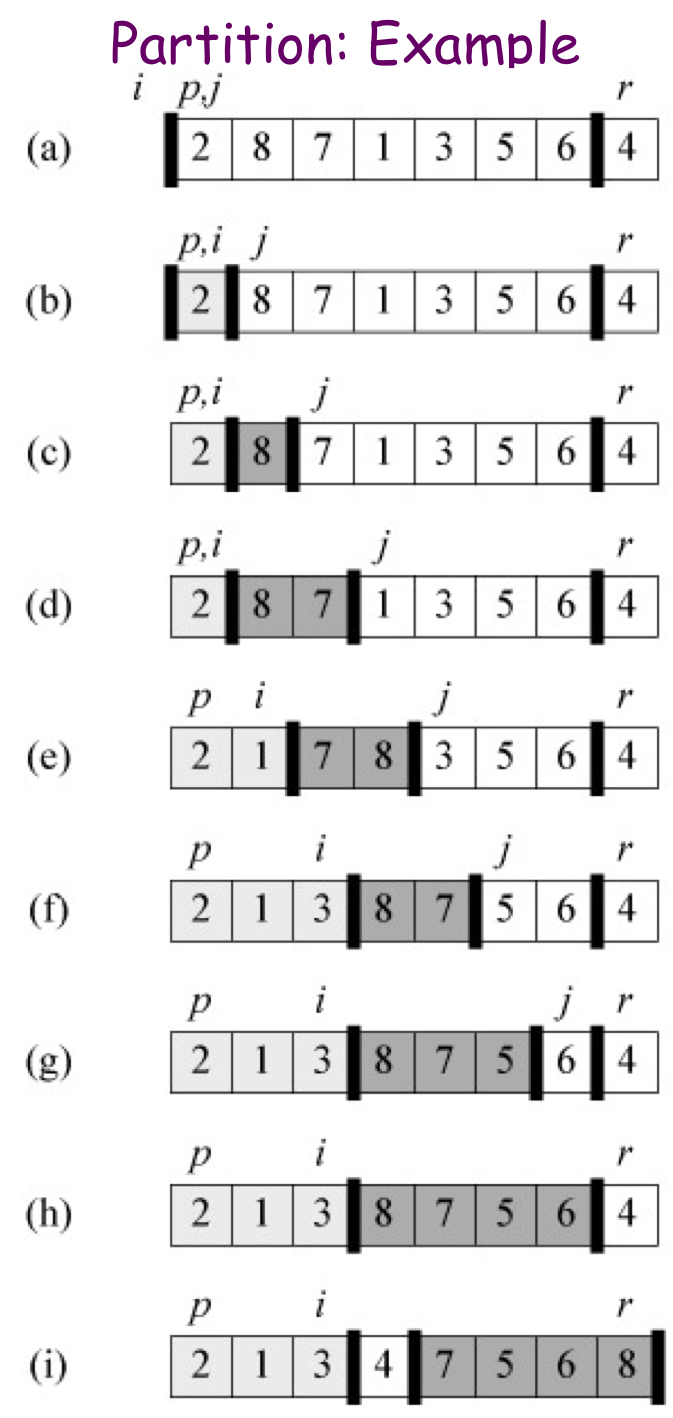
\includegraphics[scale=0.165]{images/03-partition-eg.jpeg}
    \end{center}



\end{spacing}
\end{document}
